%
% Vorlage Diplom-/Master-/Bachelorarbeit
% Norman Heino
% Version: 0.1
% Datum: 2011-03-16
% Encoding: UTF-8
%
\documentclass[% 
  parskip=half,
  ]{scrreprt} % 11pt is default

\usepackage[automark, headsepline]{scrpage2}
%\usepackage{Sweave}
%\usepackage{showframe}
\usepackage[justification=centering]{caption}
\pagestyle{scrheadings}

% Kolumnentitel in Serifenloser Schrift
\renewcommand*{\headfont}{\normalfont\sffamily\slshape}

% Alle Seiten sind rechte Seiten
\refoot[\pagemark]{\pagemark}
\rofoot[\pagemark]{\pagemark}
\rehead[]{\headmark}
\rohead[]{\headmark}
\chead[]{}
\cfoot[]{}

% „--“ zwischen Kapitel und Kolumnentitel
\renewcommand*{\chaptermarkformat}{%
  \chapappifchapterprefix{\ }
  \thechapter\autodot\enskip{--}\enskip%
}

% Use utf-8 encoding for foreign characters
\usepackage[utf8]{inputenc}

% Fonts
% Roman
\usepackage[sc]{mathpazo}
% Sans
\usepackage{avant}
% \usepackage[scaled=.95]{helvet}

% Monospaced
\usepackage[scaled=.86]{beramono}
% Mono aus den pxfonts
% \renewcommand{\ttdefault}{pxtt}
% \DeclareMathAlphabet{\mathtt}{OT1}{pxtt}{m}{n}
% \SetMathAlphabet{\mathtt}{bold}{OT1}{pxtt}{b}{n}

% Support for multiple languages
\usepackage[english,ngerman]{babel}

% Non-english bibliography
\usepackage[fixlanguage]{babelbib}
\selectbiblanguage{ngerman}

% Nicer looking fonts
\usepackage[T1]{fontenc}

% Farben
\usepackage{color}

% Conditionals
% See ftp://ftp.rrzn.uni-hannover.de/pub/mirror/tex-archive/macros/latex/contrib/xifthen/xifthen.pdf
\usepackage{xifthen}

% This is now the recommended way for checking for PDFLaTeX:
\usepackage{ifpdf}

% Document info vars
\newcommand{\diplfirstname}{Marcus}
\newcommand{\diplname}{Nitzschke}
\newcommand{\dipltitle}{Patient-centered Drug Management based on Linked Open Data}
\newcommand{\diplsubtitle}{(Arbeitstitel)}
\newcommand{\diplsubject}{Master's Thesis}

\definecolor{remcolor}{rgb}{.95,0.35,0.35}

\newcommand{\rem}[1]{\textcolor{remcolor}{\emph{#1}}}

% Hyperref
\ifpdf
%\usepackage[pdftex]{graphicx}
\usepackage[
  pdftex, 
  pdfpagelabels,
  pdfborder={0 0 0},
  pdftitle={\dipltitle},
  pdfauthor={\diplfirstname\ \diplname},
  pdfsubject={\diplsubject},
  pdfkeywords={}]{hyperref}
\else
\usepackage{graphicx}
\fi

\usepackage{graphicx}
\usepackage{epstopdf}
\usepackage{listings}
\usepackage{color}
\usepackage{url}
\usepackage{booktabs}
\usepackage{multirow}
\usepackage{rotating}
\usepackage{mathtools}

% Abbreviations
\newcommand{\linenumberstyle}{\scriptsize}
\newcommand{\lla}{\ensuremath{\longleftarrow}}
\newcommand{\todo}[1]{\marginline{\footnotesize TODO: #1}}
\newcommand{\pdfscale}{1.0} % Global scaling factor for included PDF files
\newcommand{\enlarge}{\enlargethispage{1.5em}}

% Adapt LaTeX defaults
\linespread{1.4}
\setlength{\abovecaptionskip}{.5em}
\setlength{\parindent}{1em}
\setlength{\parskip}{.2em}

% continous footnotes
\usepackage{remreset}
\makeatletter
\@removefromreset{footnote}{chapter}
\makeatother

% Adapt KOMA defaults
\setcapindent{\parindent}
\setkomafont{captionlabel}{\sffamily\bfseries}


% Listings setup
% See http://ftp.fernuni-hagen.de/ftp-dir/pub/mirrors/www.ctan.org/macros/latex/contrib/listings/listings.pdf

% define json listings
\lstdefinelanguage{json} {
  sensitive=false, 
  morestring=[b]"', 
  showstringspaces=false
}

% define turtle listings
\lstdefinelanguage{turtle} {
  sensitive=false, 
  morestring=[b]"', 
  showstringspaces=true
}

% define sparql listing
\lstdefinelanguage{sparql} {
  sensitive=false, 
  morestring=[b]"', 
  showstringspaces=true,
  backgroundcolor=\color[gray]{1.0},
  numbers=none,
  xleftmargin=0pt,
  xrightmargin=0pt,
  framexleftmargin=0pt,
  framexrightmargin=0pt
}

% set default listing style
\lstset{
  language=json, 
  basicstyle=\small\ttfamily, 
  captionpos=b, 
  % keywordstyle=\color[rgb]{0,0,0.7}, 
  % stringstyle = \color[rgb]{0,0.5,0}, 
  % identifierstyle=\color{orange}, 
  commentstyle=\color[gray]{0.5}, 
  backgroundcolor=\color[gray]{0.96}, 
  framexleftmargin=1pt,
  xleftmargin=4.4pt,
  xrightmargin=3.4pt,
  numbers=left, 
  numberstyle=\linenumberstyle, 
  frame=single, 
  aboveskip=1.3em
}

% Algorithms
% See ftp://ftp.tu-chemnitz.de/pub/tex/macros/latex/contrib/algorithm2e/algorithm2e.pdf
% \usepackage[german, algochapter, boxed, linesnumbered, vlined]{algorithm2e}
% \SetAlCapSkip{.885em}
% \SetNlSkip{1.5em}
% \SetInd{.8em}{.8em}
% \SetNlSty{linenumberstyle}{}{}
% \newcommand{\captionlabel}{\usekomafont{captionlabel}}
% \SetAlTitleFnt{captionlabel}

% Document info
\titlehead{
  \begin{center}
    \textsc{Universität Leipzig}\\
    Faculty of Mathematics and Computer Science\\
    Department of Computer Science
  \end{center}
}

% Generates the title
\title{%
\dipltitle\\%
\bigskip\usekomafont{subtitle}%
\parbox[h]{0.8\textwidth}{\begin{center}\diplsubtitle\end{center}}%
}

% Subtitle is abused as type of work
\subtitle{\usekomafont{subject}\vspace{3em}\diplsubject}
\author{}
\date{}
\publishers{
  \large\parbox{\textwidth}{%
    % \vspace*{4\baselineskip}
    Leipzig, March 2013\hfill 
    Submitted by\\
    \raggedleft
    \diplname, \diplfirstname\\
    Master's programme Computer Science
  }\\
\raggedright
\vspace{2.5cm}
\textbf{Thesis Supervisors:\\
  Prof. Dr. Klaus-Peter Fähnrich\\
  Dipl. Inf. Romy Elze
  %Department of Computer Science
}
}

\begin{document}
\selectlanguage{english}

\ifpdf
\DeclareGraphicsExtensions{.pdf, .png, .jpg, .tif}
\else
\DeclareGraphicsExtensions{.eps, .jpg}
\fi

% Seitennummerierung auf römisch
\pagenumbering{roman}

% Titelei
\maketitle

\section*{Abstract}
This thesis will present a solution for a simple way to answer several drug related questions, like ``What are the side effects of drug X?'' or ``Do drug X and drug Y interact with each other?''.
The knowledge foundation used for these queries are Linked Data knowledge bases which allow comprehensive queries over semantic data.
The presented approach provides an Application Programming Interface (API) for the different questions that allows an usage without any background knowledge about the data sources and their structures.
Additionally the predefined questions support the ``Drug Management life cycle'' introduced by the World Health Organization.
Finally the presented solution will be evaluated by integrating it in the Dispedia and DrugMan project.

%%% Local Variables: 
%%% mode: latex
%%% TeX-master: "thesis"
%%% End: 

% Zusammenfassung
%\thispagestyle{empty}


\paragraph{Keywords} Semantic Web, Linked Open Data, Drug Management

% Verzeichnisse
\setcounter{tocdepth}{1}
\tableofcontents

% Ab nächster Seite
\clearpage
% Seitennummerierung auf arabisch
\pagenumbering{arabic}

% \begin{abstract}
% \end{abstract}

\chapter{Introduction}
\label{cha:introduction-1}

\section{Subject}
\label{sec:subject}

The prescription and application of drugs in health care is one of the most important parts in the healing process of  a patient.
If this process is not managed accurately consequences from financial losses to  human harms are possible.
In Germany estimations state that annually 25,000 patients die because of medication errors \cite{pharzeit10} (status 2010).
Managing drugs means to support the different phases drugs passes during the healing process.
The \textit{World Health Organization} (WHO) published a Drug Management Cycle which defines four different phases \cite{who2004}.
Details about this Drug Management Cycle are given in section \ref{sec:drug-management}. 
An important base to implement a proper drug management and therefore to avoid the problem of medication errors is that all available knowledge about drugs and their characteristics is freely accessible and usable.
Especially in the biomedical domain the role of ontologies for structuring such knowledge is still growing since decades.
And in the last years a trend towards open access policies that on the one hand make the respective knowledge available freely and on the other hand allows the further use of these ontologies and the provided data is noticable.
Newer examples for such projects that either provide these ontologies or use the free access for other use cases is the \textit{Linking Open Drug Data} (LODD) \cite{jentzsch2009linking} or BioPortal \cite{whetzel2011bioportal} project.
%This process of publishing medical -- drug related -- data has already started in the last years with projects like \textit{Linking Open Drug Data} (LODD) \cite{jentzsch2009linking} or BioPortal \cite{whetzel2011bioportal}.
LODD is a project that links the knowledge of several vocabularies by recognizing common entities.
The additional gained knowledge in form of so called ``linked data'' is again provided freely under an open access policy.
More details about this approach are given in section \ref{sec:linked-open-data}.
The second project -- BioPortal -- offers a platform where people or projects serve their biomedical ontologies and knowledge bases.
These knowledge bases can in turn be mapped so that the same entities in different vocabularies are identified.
%That is important because so it is possible for everyone to build third-party applications on top of this data.
Although it is possible to build third-party applications on top of this data, such applications are very rare at this time.
In the case of LODD only small projects exist like DiseaseCard \cite{oliveira2004diseasecard} or Pharmer \cite{khalili2013pharmer}.
The former one is graph-based browser that visualizes associated entities of other knowledge bases regarding a certain disease.
The latter one -- Pharmer -- is a proof of concept for the authoring of semantic prescriptions.

Besides these third-party projects mainly clinical applications implement specific drug related functionalities.
For example a \textit{Patient Information System} stores all the details about the prescribed drugs of a certain patient.
Therefore a nurse could be supported in the process of drug application by offering information about the route of application or the maximum dosage.
Another application, like a \textit{Computerized Physician Order Entry System} that selects and prescribes drugs, could check for interactions of the drugs that are going to be prescribed.
And for both of the applications the side effects of a certain drug may be of interest.
These examples show that many different medical applications implement drug related functionalities.
And many of them also share the same requirements regarding the used data sources because there is a set of common questions, like \textit{``What are the side effects of drug X?''}.
But ignoring these shared requirements, many of the applications provide their own -- mostly proprietary -- knowledge bases.

A comparable situation on the data level of another domain was recently solved.
The Wikidata project ``centralizes access to and management of structured data'' \footnote{\url{https://www.wikidata.org/wiki/Wikidata:Main_Page} (last access Sept 18, 2013)}.
It solves the problem that many different Wikipedia provided common data about the same entities, e.g. the population of countries.
Now Wikidata centrally provide this data through a common interface and the different Wikipedia refer to this source.
In consequence there exist only one place where the data has to be updated and maintained.


% \begin{itemize}
% \item verschiedene anwendungen im  bereich arzneimittelmngtm
% \item überschneidende funktionalität
% \item 
% \item keine endanwendungen auf lodd basierend bekannt
% \end{itemize}

\section{Problem}
\label{sec:problem}

In section \ref{sec:subject} the diversity of applications that implement drug related functionalities was mentioned.
This goes along with the fact that multiple knowledge bases are used which actually should provide the same data. 
This leads to several problems.

The first problem -- insufficient integration -- follows from the different scopes and the different expressivity of the knowledge bases.
This means there are many knowledge bases for special domains like side effects or alternative medicine.
But if one knowledge base wants to use the data of another special domain this is usually not possible, for instance because of an insufficient semantic integration.
This means that term $x$ in knowledge base $X$ does not implicitely refer to the same object as term $x$ in knowledge base $Y$.
Therefore the knowledge bases have to provide the data on their own.

This is the starting point of the next problem: redundancy.
Many drug related knowledge bases include a set of common facts that are essential for this domain, like the code of the \textit{Anatomical Therapeutic Chemical Classification System} (ATC).
So this is a common \textit{``Don't repeat yourself''} problem.
A side effect of this problem is the higher chance that a given statement of a knowledge base is wrong or not up-to-date anymore.

So the third problem is the correctness of the knowledge.
Proprietary knowledge bases generally have to deal with a strong limited number of people validating the data.
In contrast open projects like Wikipedia are considered as ``self-healing'' information systems because of the high number of volunteers that report and correct data errors.
To transfer this phenomenon to medical data it is unimaginable that everyone could edit such important information, but reporting errors would be a strong impact nonetheless.
%While the number of persons that validate the data of a proprietary knowledge source is limited, projects like Wikipedia has shown the power of an open review process in the last years.

Section \ref{sec:subject} presented two third-party applications using open data as their knowledge sources.
A common problem using these data sources is the extensive schema knowledge that is required to use the data efficiently. 
Besides the information about the usage of the given interface the developers are often forced to understand the structure of the data to perform their respective queries.
This can be a deal-breaker for developers and therefore for innovative applications.
% \begin{itemize}
% \item unterschiedliche implementierungen
% \item unters. quellen
% \item ausgesagt werden soll aber das selbe
% \item 
% \item umfangreiches schemawissen nötig um anfragen an lod stellen zu können
% \end{itemize}

\section{Motivation}
\label{sec:motivation}

If the given problems of section \ref{sec:problem} could be solved this would lead to a better data quality in the first place.
Data quality contains in this context the expressivity, completeness and correctness of the knowledge.
Medical applications would benefit from this improvement by getting a proper knowledge foundation.
Following from that this would lead to unified, more well-grounded decisions for drug related questions.
By supporting physicians, nurses, pharmacists and even the patient itself this would hopefully avoid some of the prescription errors that are made during the healing process of a patient.

Solving the problem that developers often have to know the schema of a certain knowledge base the consequence would be a reduced starting barrier for application developers.
Instead of knowing about the whole schema of a knowledge base, only the knowledge about using the given interface would be required.
Probably this would lead to many interesting applications on top of the given data.
And by a growing number of applications using these data sources more and more feedback would be flow back to improve the knowledge bases in turn.

% \begin{itemize}
% \item durch einheitliche schnittstelle soll datenqualität vereinheitlicht werden
% \item einstiegsbarriere für neue anwendunge senken (cpoe)
% \item 
% \item vereinfachen der möglichkeit wissen aus lodd zu nutzen
% \item (praxiseinsatz von lodd)
% \end{itemize}

\section{Objectives}
\label{sec:objectives}

Emerged from the motivation, this thesis shall proof that Linked Open Data is an appropriate knowledge source for drug management tools.
For this purpose a web-based \textit{Application Programming Interface} (API) will be provided.
This API will support the process of answering drug related questions according to the WHO drug management life cycle.
This is achived by offering several API endpoints -- e.g. for drug-drug interactions -- that gather information from several semantic knowledge bases and return the merged results.
One design goal is the simplicity of the API to reduce the starting barrier of developing new applications based on the given interface.
More details about the implementation process are described in chapter \ref{cha:methods}.

This thesis shall also provide two use cases where the usage of the API will be demonstrated and evaluated.
The first use case is the integration in Dispedia -- an information system in the complex field of rare diseases \cite{elze2013dispedia}.
The main purpose here is the integration of the drug-drug interaction endpoint.
The second use case is a personal drug management portal built around this API to support privat persons managing their prescribed drugs.
This use case shall demonstrate the other available endpoints of the provided interface.
Chapter \ref{cha:evaluation} will offer more information about this evaluation process.

% \begin{itemize}
% \item bereit\-stellen einer API zur unter\-stützung des drug manage\-ment cycles basierend auf lod(d)
% \item evaluation anhand verschiedener anwendungsfälle
% \begin{itemize}
% \item dispedia
% \item eigenes portal zur arzneimittel-verwaltung
% \end{itemize}
% \end{itemize}

%%% Local Variables: 
%%% mode: latex
%%% TeX-master: "../thesis"
%%% End: 


\chapter{Preliminaries}
\label{cha:prelims}

\section{Drug Management}
\label{sec:drug-management}

To get a better understanding what the term Drug Management stands for it is essential to clearify the term Management at first.
Management comprises the non-executing tasks of a certain domain... \todo{}
The term Drug Management was adopted by the WHO in their publication about managing drugs at health centres \cite{who2004}.
The term management is defined in their publication as follows: 
\begin{quote}
  Management is the act or art of being responsible or in charge and conducting or supervising something (e.g. a health centre pharmacy, business, public undertaking) with a degree of skill and address. It is the judicious use of means to accomplish an end (i.e. public health).
\end{quote}
With this definition in mind the question can be answered why it is useful to manage drugs.
Refering to the WHO there are three main reasons:
\begin{enumerate}
\item ``Firstly, drugs are part of the link between the patient and health services.''\\
  This is the most trivial reason that addresses the direct influence of drugs to the patients health state. If drugs are not managed properly the success of the treatment process is imperiled. 
\item ``Secondly, poor drug management [...] is a critical issue, but major improvements are possible that can save money and improve access.''\\
  Besides the medical benefits, a proper drug management can also result in financial advantages. These can be achived by an improved selection and procurement of the required drugs.
\item ``Finally, drugs are no longer the responsibility of health workers only.''\\
  blah \todo{}
\end{enumerate}

\begin{figure}
  \centering
  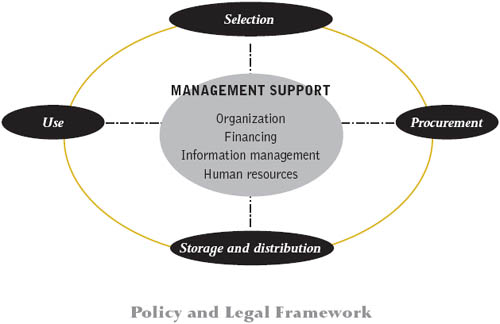
\includegraphics[scale=2]{preliminaries/life_cycle.jpg}
  \caption{WHO drug management life cycle}
  \label{fig:life_cycle}
\end{figure}
The WHO proposes a drug management life cycle which is the foundation to implement a proper drug management at a certain institution.
This life cycle which is shown in figure \ref{fig:life_cycle} contains four phases which are described shortly in the following listing:
\begin{itemize}\todo{}
\item Selection
\item Use
\item Procurement
\item Storage and Distribution
\end{itemize}
According to the WHO these phases ``are interlinked and are reinforced by appropriate management support systems (i.e. tools)''.
The API which is developed by this thesis is settled up in this category of support systems.

One point has to be remarked regarding the scope of the WHO recommendations.
Althought the cited publication addresses health centres, recommendations like the life cycle are easily adoptable to other areas, e.g. private healthcare.

\section{Semantic Web}
\label{sec:semantic-web}
The ongoing growth of digital data in the past years has revealed many shortcomings that occur with these amounts of data.
Fields of research like \textit{Big Data} also show the importance of managing these amounts of data efficiently.
One key issue since years is the distinction between syntactically and semantically processable data.
Tim Berners-Lee proposed in 2001 a model to describe specific data statements in a better way.
This approach was called \textit{Ressource Description Framework} (RDF) and is one important part of the Semantic Web Stack.
This stack combines several technologies and standars that are necessary to transfer the syntactic web to a semantic web.
The Semantic Web Stack is illustrated in figure \ref{fig:sem_stack}.
\begin{figure}
  \centering
  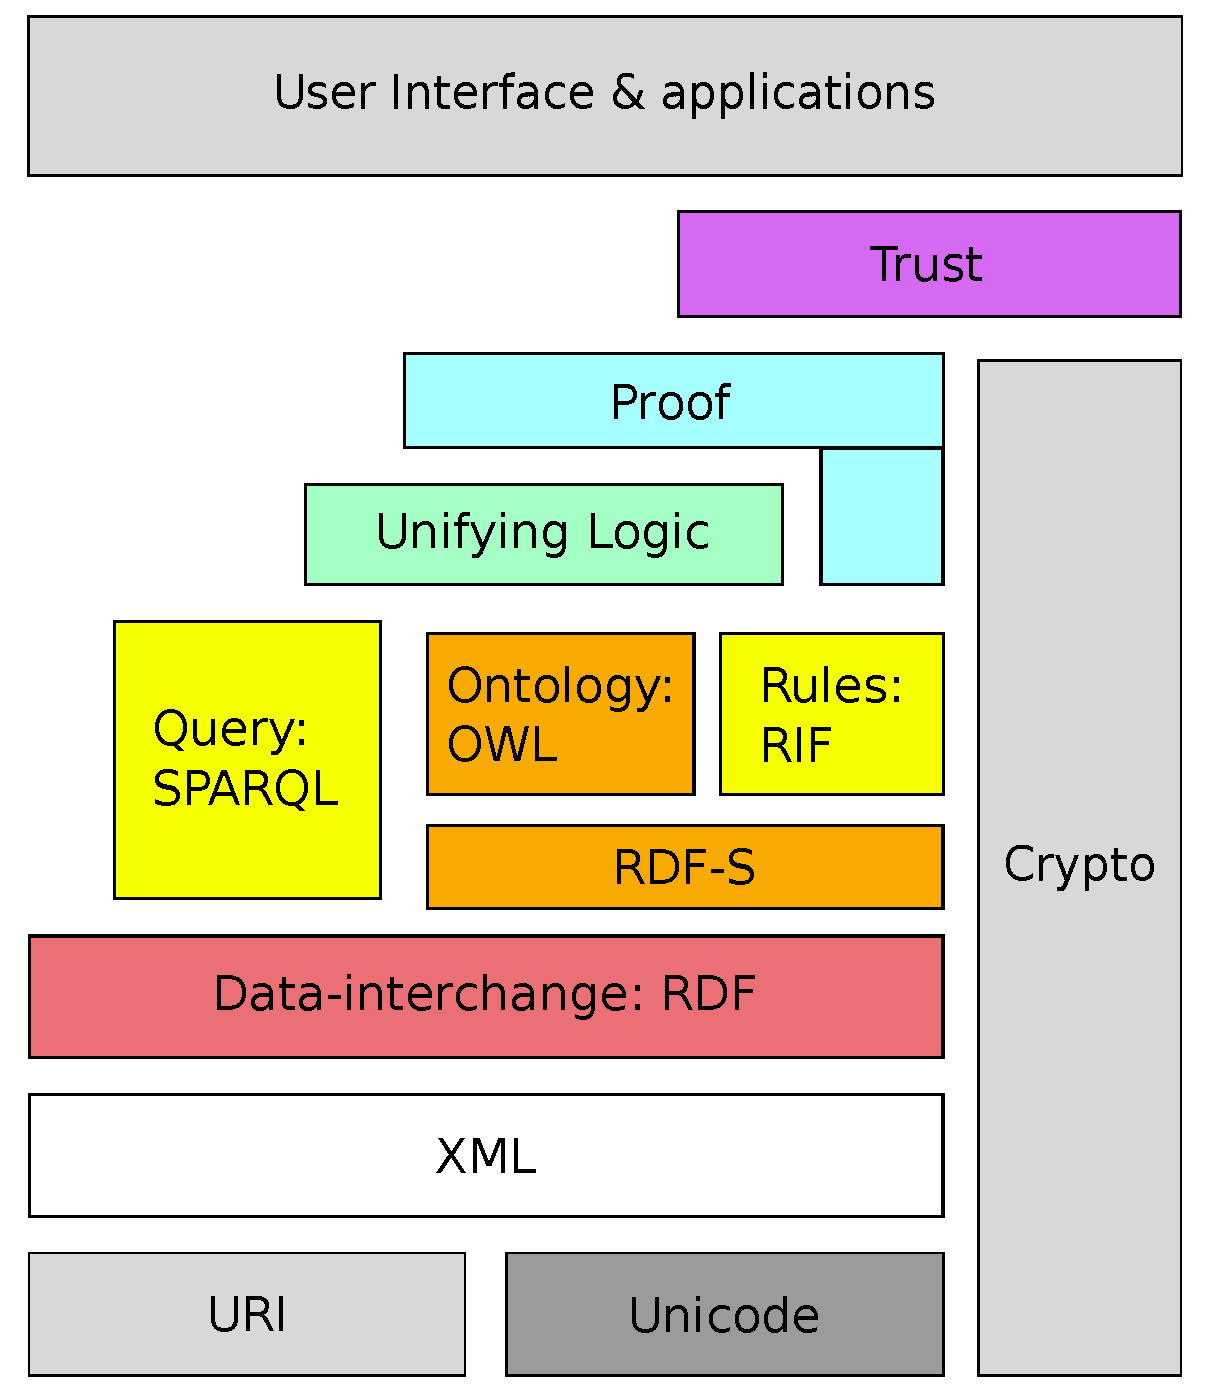
\includegraphics[scale=0.3]{preliminaries/semweb_stack}
  \caption{Semantic Web Stack}
  \label{fig:sem_stack}
\end{figure}
The advantages of a semantic web are numerous.
The main advantage is that the information are not only machine readable but machine processable.
This entails other improvements like reasoning that transfers implicit knowledge into explicit.

The following paragraphs will describe the most important technologies and standards of the Semantic Web Stack that are necessary for this thesis:

At the lowest level of the stack there are the Uniform Resource Identifier (URI).
A URI identifies a specific resource, e.g. a car.
For several other domains there already exists such concepts as URIs.
For example the Uniform Resource Locator (URL) identifies web sites or an International Standard Book Number (ISBN) identifies books.
The URI itself is just a set of characters that can be additionally divided into five segments: scheme, authority, path, query and fragment.
An example of such a URI would be: \texttt{http://example.com/Alice}.
This URI would describe the resource ``Alice''.

Based on the identification of resources, the already mentioned Resource Description Framework has the goal to describe these resources.
Therefore RDF is one of the most important concepts of the Semantic Web Stack.
The approach of RDF to model knowledge is to express statements as triples.
This is tight to how natural language is mostly constructed.
Obviously that is why the components of the triple use the well known names of \textit{Subject, Predicate} and \textit{Object}.
Figure \ref{fig:sem_rdf} shows an example triple.
The subject of such a triple has to be always an URI, same belongs to the predicate.
An exception is the object which can be additionally a literal.
A literal is a direct information typed in a specific way, e.g. as date or simply text, which refers to no other resource.
For more advanced models it is possible to describe the subject and object in a anonymous way, without a concrete entity.
These anonymous resources are called blank nodes, but will be without broader relevance for this thesis.
At the end one important distinction has to be made about RDF.
Often RDF is getting confused with RDF/XML -- a notation of RDF statements.
While RDF itself only describes how to model information, several RDF notations exist that express these information in several ways.
Examples for such notations besides the already mentioned RDF/XML is N-Triples, Turtle or JSON-LD.

\begin{figure}
  \centering
  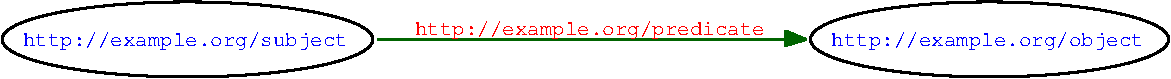
\includegraphics[width=\textwidth]{preliminaries/semweb_rdf1}
  \caption{Example of a RDF triple}
  \label{fig:sem_rdf}
\end{figure}

On top of RDF the Semantic Web Stack levels SPARQL, an RDF query language.
SPARQL enables comprehensive queries over a knowledge base built on RDF.
SPARQL itself uses many well known keywords from SQL, but because of the graph structure of RDF and therefore of the triple stores the languages naturally differ.

Given the following two triples in Turtle notation:
\begin{lstlisting}[numbers=none,label=turtle]
@prefix ex: <http://example.com/>.
ex:anna ex:name ``Anna''.
ex:bob  ex:name ``Bob''. 
\end{lstlisting}

Then the following simple SPARQL query would return the result ``Bob''.
\begin{lstlisting}[numbers=none,label=sparql]
SELECT ?name
WHERE {
  ex:bob ex:name ?name.
}
\end{lstlisting}

With SPARQL 1.1 so called \textit{Federated Queries} were introduced.
These Federated Queries are Statements that are queried against multiple (federated) SPARQL endpoints.
This is a key feature for an easy integration of several RDF graphs.

\section{Linked Open Data}
\label{sec:linked-open-data}
As described in the previous section RDF statements spans a graph of triples.
Thereby, each knowledge base spans their own graph.
Examples for large knowledge bases are DBpedia\footnote{\url{http://dbpedia.org}}, LinkedGeoData\footnote{\url{http://linkedgeodata.org}} or Drugbank.
\textit{Linked Data} in general now describes the situation that entities of one knowledge base link to entities of another knowledge base.
For example an entity of DBpedia about a drug could link to the same entity in Drugbank for further information.
If the mentioned knowledge bases are freely available and usable then this is called \textit{Linked Open Data}.

Tim Berners-Lee proposed some rules that state whether a data source is Linked Open Data, or not.
These rules are:
\begin{enumerate}
\item Use URIs to denote things.
\item Use HTTP URIs so that these things can be referred to and looked up ("dereferenced") by people and user agents.
\item Provide useful information about the thing when its URI is dereferenced, leveraging standards such as RDF, SPARQL.
\item Include links to other related things (using their URIs) when publishing data on the Web.
\end{enumerate}

Further, Berners-Lee categorizes Linked Open Data on the basis of a five star rating.
Therefore the more a knowledge base follows these principals the more stars it earns.
\begin{itemize}
\item \textbf{1 star} - Available on the web (whatever format) but with an open licence, to be Open Data
\item \textbf{2 stars} - Available as machine-readable structured data (e.g. excel instead of image scan of a table)
\item \textbf{3 stars} - as (2) plus non-proprietary format (e.g. CSV instead of excel)
\item \textbf{4 stars} - All the above plus, Use open standards from W3C (RDF and SPARQL) to identify things, so that people can point at your stuff
\item \textbf{5 stars} - All the above, plus: Link your data to other people’s data to provide context
\end{itemize}

In conjunction with SPARQL this leads to large federated collections of knowledge that are comprehensively queryable.
Figure \ref{fig:lod_cloud} gives an overview over the Linked Open Data cloud in 2011.
But this kind of figure will end soon because of the rapidly evolving number of data sets.
\begin{figure}
  \centering
  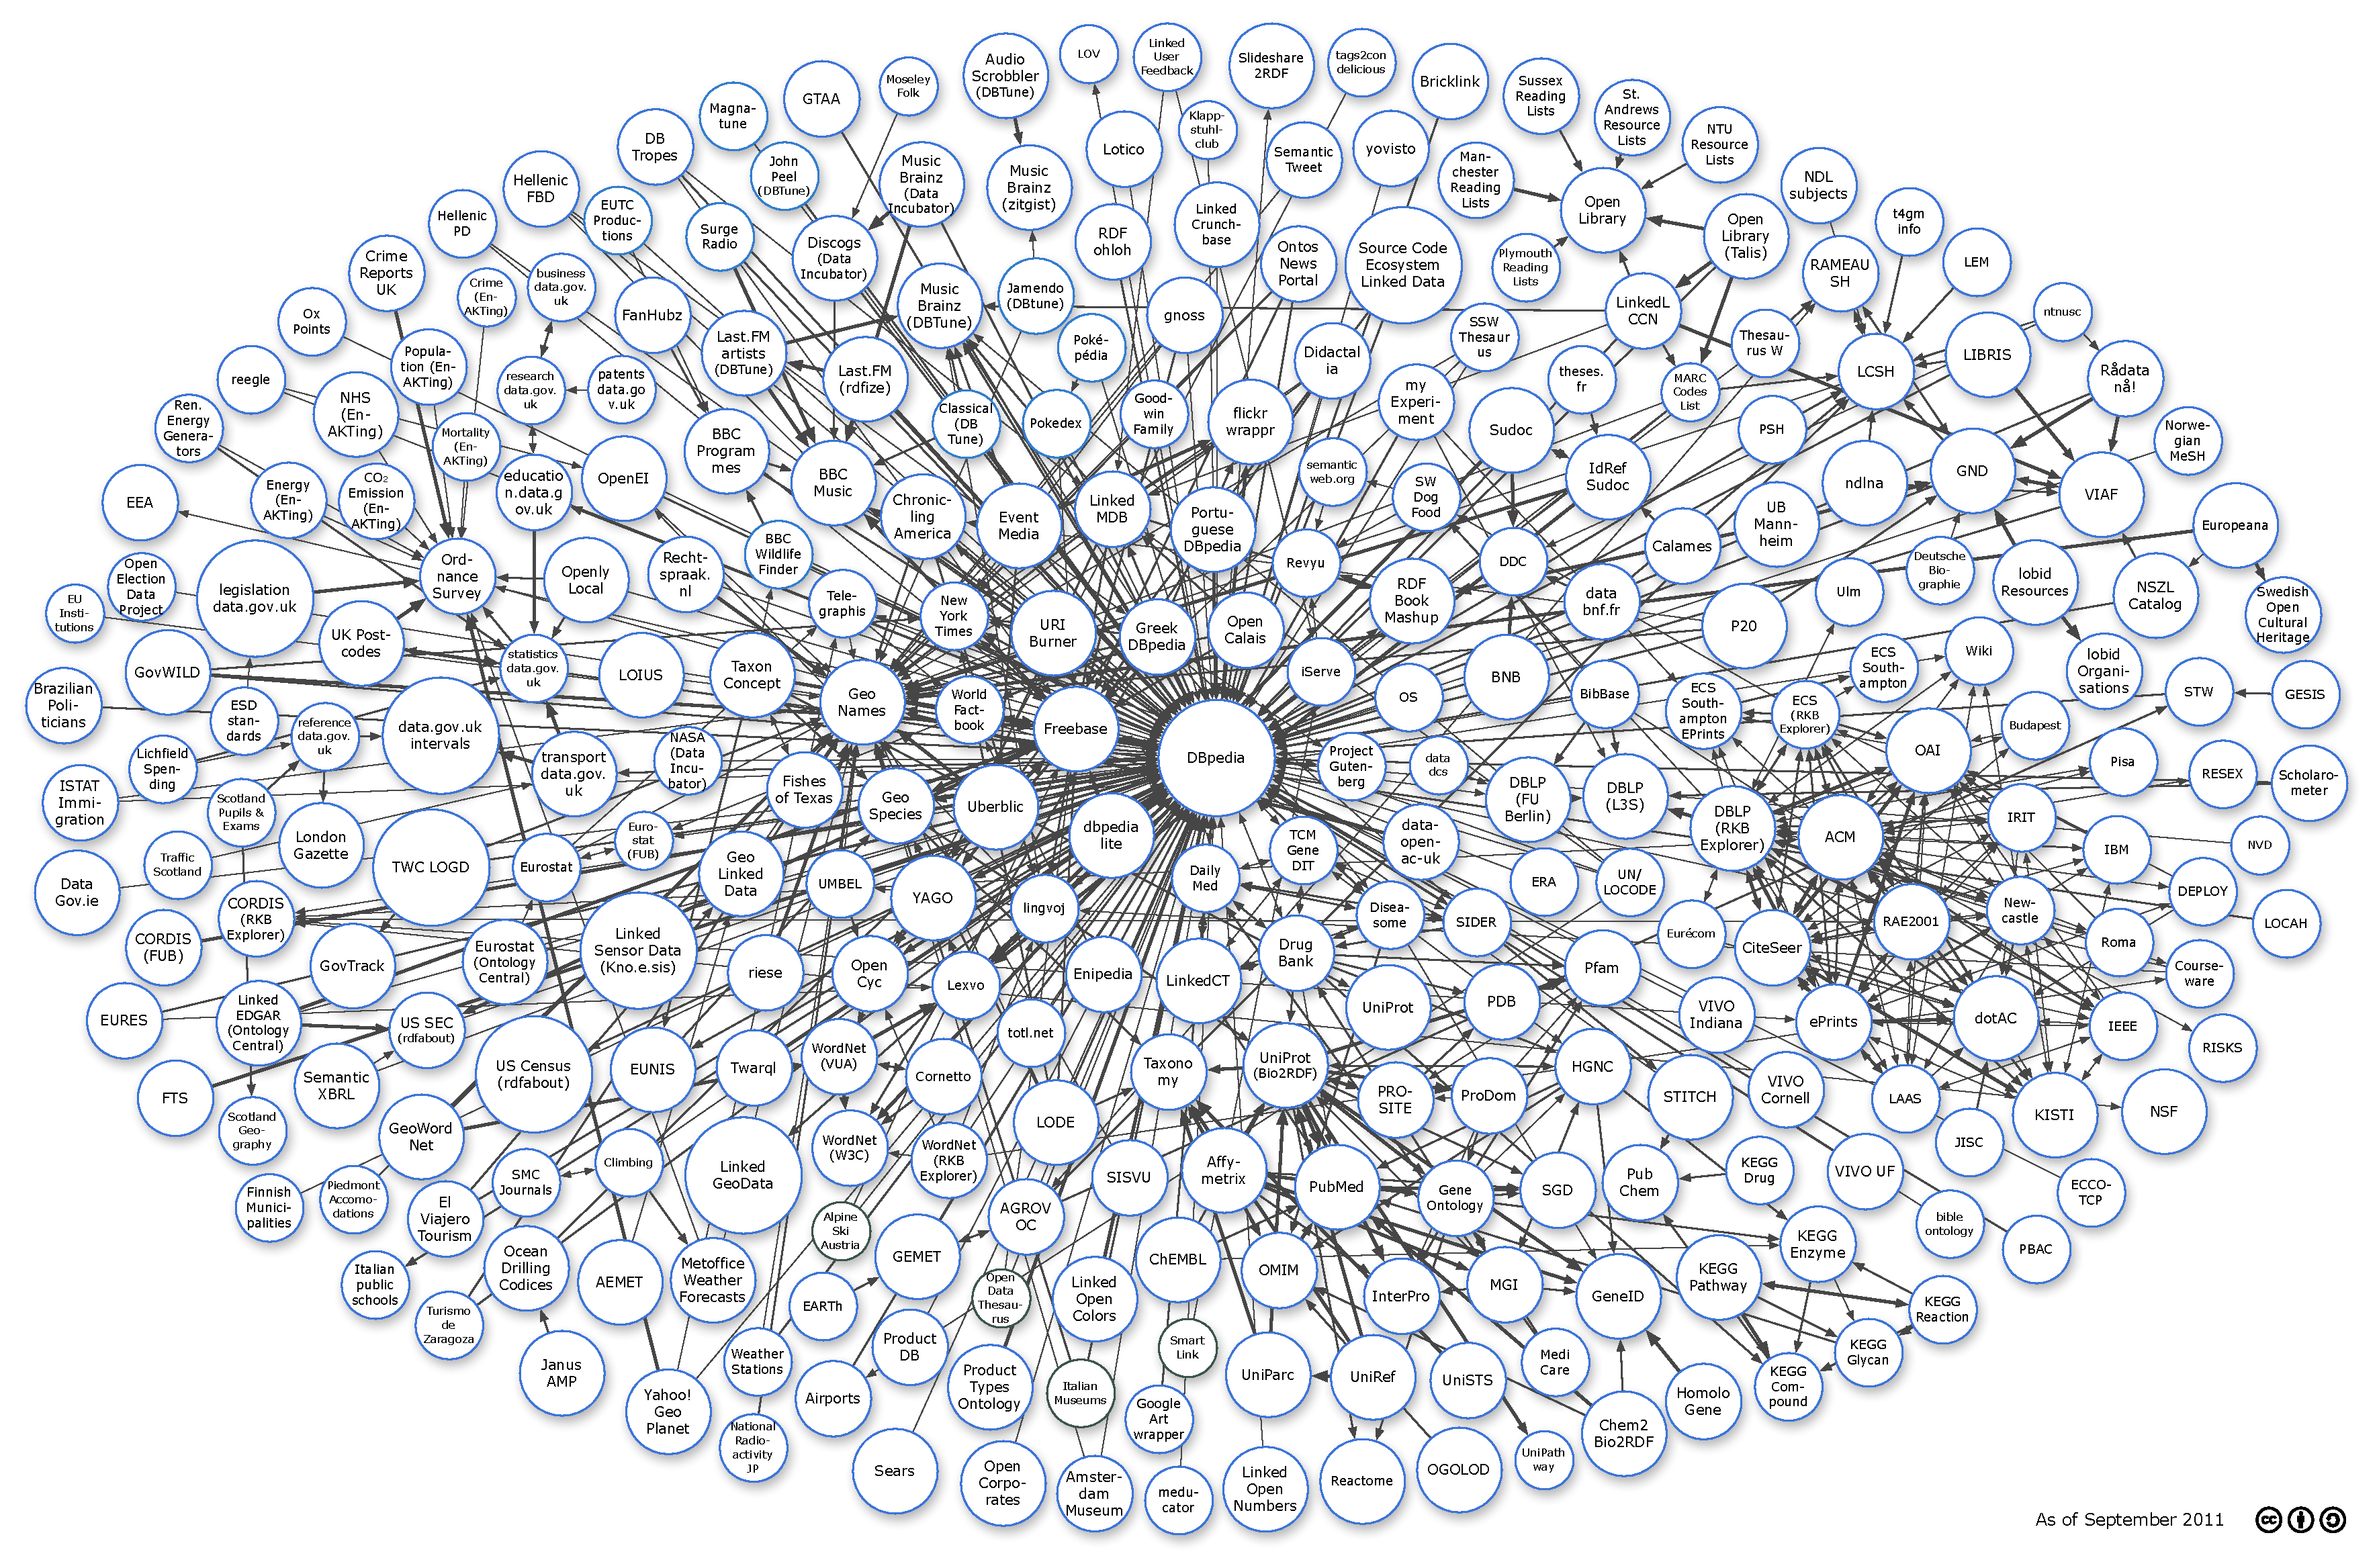
\includegraphics[width=\textwidth]{preliminaries/lod-cloud}
  \caption{Linking Open Data cloud diagram, by Richard Cyganiak and Anja Jentzsch. http://lod-cloud.net/}
  \label{fig:lod_cloud}
\end{figure}

%%% Local Variables: 
%%% mode: latex
%%% TeX-master: "../thesis"
%%% End: 


\chapter{Methods}
\label{cha:methods}

\begin{itemize}
\item sparql federated queries nicht überall unterstützt -> construct und dann lokales mergen
\item übersicht datensätze
  \begin{itemize}
  \item tabellarisch/grafisch
  \item proprietäre quellen die nicht verwendet werden konnten
  \begin{itemize}
  \item senger et al
  \end{itemize}
  \end{itemize}
\end{itemize}

%%% Local Variables: 
%%% mode: latex
%%% TeX-master: "../thesis"
%%% End: 



\chapter{Evaluation}
\label{cha:evaluation}

The evaluation of SEDRI has the goal to test how well it can be integrated in different projects with different use cases, based on different programming languages and so on.
This thesis will evaluate SEDRI by integrating it in two projects: Dispedia and DrugMan.

\section{Dispedia}
\label{sec:dispedia}
% \begin{itemize}
% \item Anwendungsfälle und Vorgehen beschreiben
% \end{itemize}

\subsection{Introduction}
\label{sec:introduction}
% \begin{itemize}
% \item konzept prop, propcomp
% \item patient medikationsplan
% \item unterscheidung drug/drug product
% \end{itemize}

``The Dispedia Framework is an information system in the complex field of rare diseases. The goal of the system is to harmonize social care conditions and health care conditions with the focus on personalization and patient autonomy.'' \cite{elze2013dispedia}\\
Dispedia is based on several ontologies and uses Linked Open Data e.g. for additional information about diseases or drugs.
The following paragraph will describe some of the core concepts of Dispedia which are essential for the integration of SEDRI.

Maybe the most important core concept are \textit{Proposals}.
A proposal is a possibility of a physician to offer several therapeutic activities to a patient.
In the Dispedia model a proposal represents a frame for multiple proposal components.
A proposal component in turn contains the mentioned therapeutic activities like prescribing drugs, medical devices or other services.
Proposal components act like bricks which can be assigned to different proposals.
This is a flexible way to create treatment offers.
Proposals are assigned to patients.
The relationship proposal -- patient is $n:m$ which means that it is possible to assign a proposal to multiple patients and that a patient can hold multiple proposals.\\
Besides these proposals a patient can receive several products or services, like drug products or a physiotherapy.
This is relevant for the integration of SEDRI because in that way there are two ways how a patient can take drugs.
First by accepting a proposal and second by ``receiving'' a drug product on their own.\\
The third important concept is the distinction between a drug and a drug product.
As described in the last sentences a patient can receive a drug product.
A drug product is a concrete commercial product distributed by a pharma company.
These products include an active ingredient which is the ``drug'' in the Dispedia sense.
An example of the distinction may be the drug product ``Ibuflam'' and the drug ``Ibuprofen''.

\subsection{Integration of SEDRI}
\label{sec:integration-sedri}

The integration point of SEDRI in Dispedia is the possibility to propose a specific drug to a patient.
In that case SEDRI is used to check the proposed drugs for possible drug-drug interactions.
In detail there are three integration points which are described in the following listing in more detail: 
\begin{itemize}
\item \textit{Check A}: The first integration is when a proposal component is created.
Each proposal component can contain multiple drugs.
If such a proposal component is created or modified then the containing drugs are tested for possible interactions.
In this case Dispedia has nothing to do than calling SEDRI with the appropriate drug codes that are stored in the system and to process the results.
\item \textit{Check B}: The second integration is implemented in the logic of proposals.
As the introduction about Dispedia described each proposal can contain multiple proposal components which theirselves contains drugs.
In this scenario it is possible that a physician proposes a specific proposal including multiple components where each component itself contains no interactions but the components among each other contains interactions.
To prevent such a scenario the components of a proposal are tested for interactions on creation and modification of the proposal.
\item \textit{Check C}: The third integration of the drug-drug interaction endpoint is implemented in the patient proposal allocation.
If a physician allocates several proposals to a patient, these proposals will be checked against the current medication of the patient.
This prevents patients to get interacting drugs in their medication plan.
In this third case one difference to the other two implementations has to be considered.
Because the items of the medication plan of the patient are drug products in the meaning of Dispedia the active ingredient of this drug product has to be received.
In the other two cases the drugs could be directly compared because the proposals and proposal components contain no drug products but drugs.
\end{itemize}
If in one of those cases an interaction is detected the details of the interaction are saved in relationship to the corresponding instance of the proposal or proposal component.
This allows the system to provide these information in other use cases.
For example when a patient decides to accept or decline a proposal the possible interaction information of the third check can be provided.
In this case an additional call of SEDRI is not necessary.

\begin{figure}
  \centering
  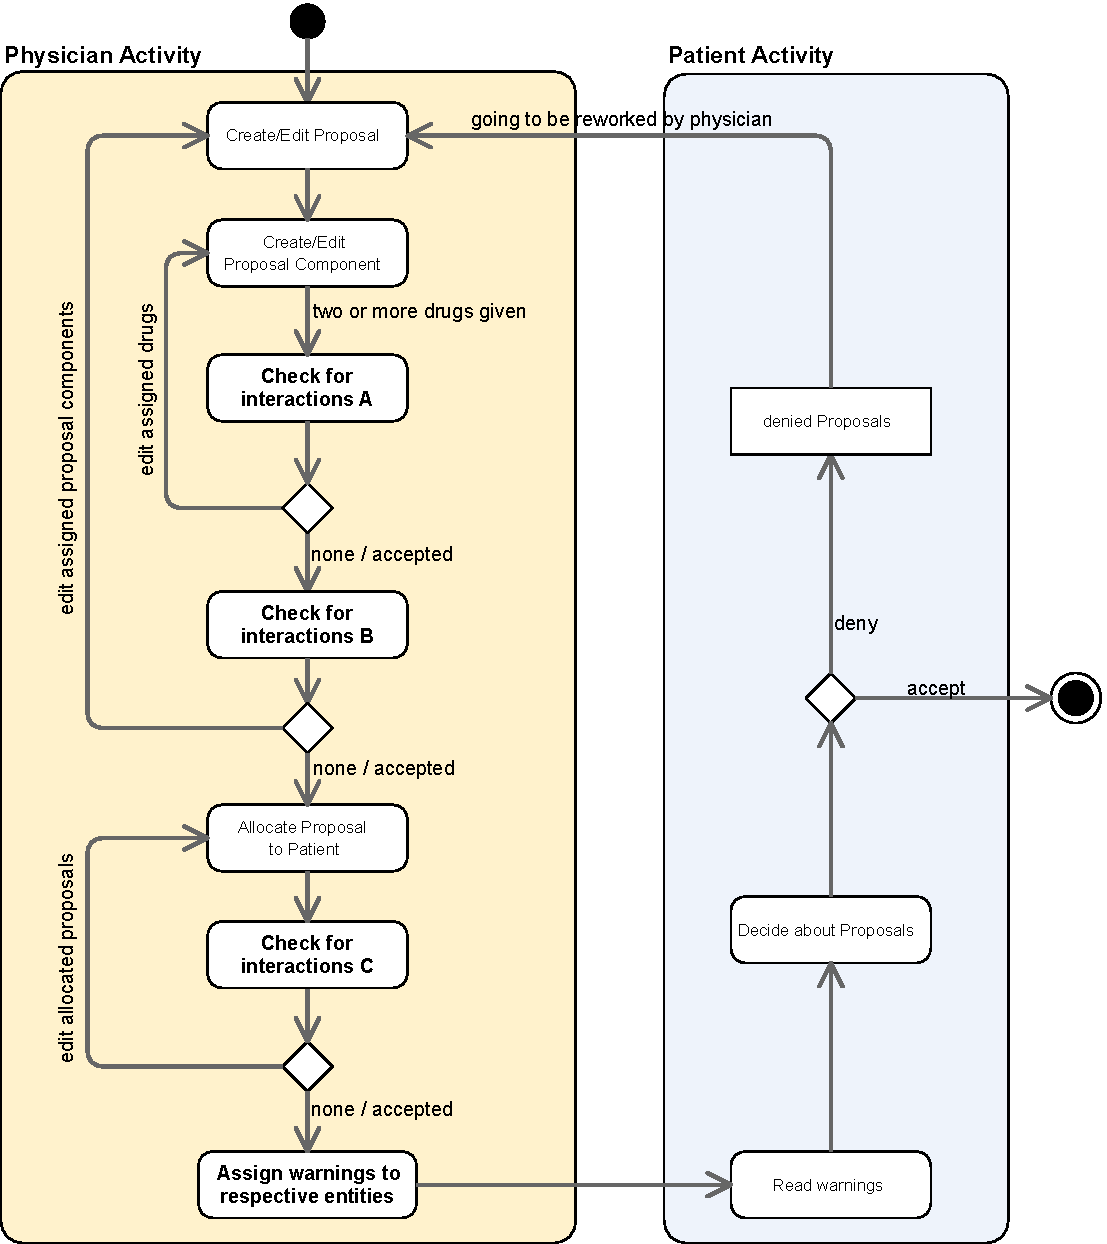
\includegraphics[scale=0.49]{evaluation/Dispedia_Integration_activity.pdf}
  \caption{Activity diagram of Dispedia proposal workflow}
  \label{fig:dispedia_activity}
\end{figure}
Figure \ref{fig:dispedia_activity} gives a graphical overview of the typical proposal workflow in Dispedia and where SEDRI is used.\\
The workflow is divided in the physician's activity and the patient's activity.
The beginning of the workflow is the creation of a new proposal by a physician.
If there are already existing proposal components then several of these components can be added to the new proposal.
Otherwise or additionally it is possible to create new proposal components.
These proposal components may contain drugs or other therapeutic activities as described in the previous introduction section.
If a new proposal component was created the included drugs will be tested for drug-drug interactions by SEDRI (\textit{Check A}).
After all desired proposal components are added to the proposal and the proposal is saved, the second call of SEDRI (\textit{Check B}) is executed.
Now the new proposal can be allocated to several patients.
In this step SEDRI executes the third check (\textit{Check C}).
With the completed proposal allocation the activity of the physician is finished.
The patient's activity starts with taking note about the given drug-drug interactions in their allocated proposals.
Based on these information the patient can accept or decline a given proposal.
In case of accepting the proposal the workflow ends.
Otherwise the physician is notified that a proposal has been declined and the physician is now able to rework the proposal.
This means the workflow starts the next iteration.

\begin{figure}
  \centering
  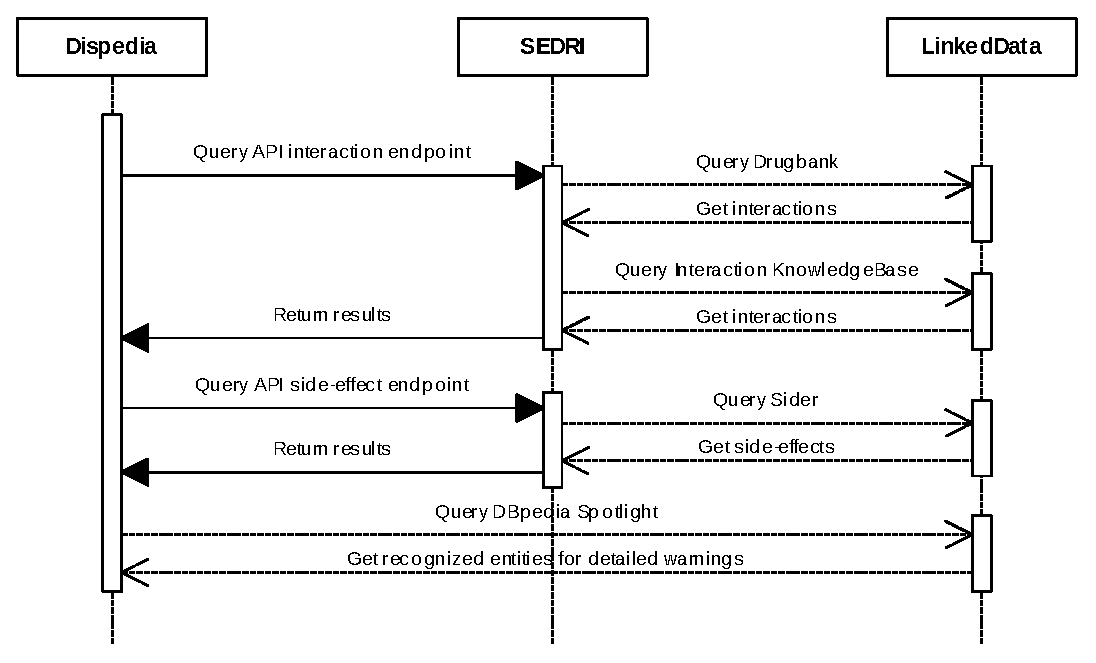
\includegraphics[width=\textwidth]{evaluation/LODD_Wrapper_Sequences.eps}
  \caption{Sequence diagram of Dispedia and SEDRI information flow}
  \label{fig:dispedia_sequence}
\end{figure}
Figure \ref{fig:dispedia_sequence} gives an overview of the information flow between Dispedia, SEDRI and the Linked Open Data cloud.
It illustrates how Dispedia is calling SEDRI for two use cases, interactions and side effects.
The latter one was not in the scope of this evaluation and is not implemented yet.
The calls to SEDRI are synchronous which means Dispedia has to wait until the results are delivered by SEDRI to work on further.
SEDRI itself calls different Linked Data sources asynchronously.
After the results are delivered by SEDRI, the diagram shows that Dispedia continues processing these results.
In this case Dispedia calls the DBpedia Spotlight annotation service\footnote{\url{http://dbpedia-spotlight.github.io/demo/} (last access Sept 09, 2013)} which extracts several entities from a given text and links them to their DBpedia resources.
This can improve the given warning messages by much more information.

\section{DrugMan}
\label{sec:portal}

\subsection{Motivation}
\label{sec-1}

Spoken for Germany there is a static rise in the last years of multiple morbidities of patients.
These often imply automatically that the regarding patient takes also multiple drugs.
In the case of five or more medications this is called \textit{Polypharmacy} \cite{montamat1992overcoming}.
Besides the fact of the multiple medications this term stands also for the unnecessary prescription of drugs which may lead to several issues.

A general issue of polypharmacy is that it is hard for patients as well as physicians or pharmacists to keep track of all the currently prescribed medications.
Additionally the patient can buy several prescription free drugs that also could lead to issues with the other prescribed drugs.
If this overview of all the medication can not be preserved then different physicians may prescribe independently their drugs what often leads to overlapping prescriptions or interacting drugs in the medication of the patient.

Another problem that DrugMan is facing is the low self-determination of people during pharmacotherapy.
This self-determination covers the confirmability and information procurement in the process of pharmacotherapy.
One example where these two values are lacking are drug-drug interactions.
If a patient is taking five drugs, which is the lower limit of polypharmacy, then there are ten possible drug-drug interactions that a patient has to test if he wants to know whether his medication includes interactions or not.
These information about possible interactions are provided by the instruction leaflet.
But these information -- in the case of Germany -- doesn't name any specific drug names but only drug classes.
So without any expert knowledge it is nearly impossible for a patient to get any concrete information about possible drug-drug interactions.
And in the case that the information would be available it is cumbersome for a private person to test all the possible combinations of drugs.
% \begin{itemize}
% % \item schwer für ärzte überblick über verfügbare medikamente am markt zu behalten
% % \item oft bilden sich aus erfahrung paare von medikamenten zu gegebener krankheit die nur selten dann erneuert werden (Quelle oä?)
% % \item 
% \item ärzte verschreiben oft unabhängig voneinander medikamente
% \item patient hat möglichkeit rezeptfreie medikamente zusätzlich einzunehmen
% \item bpz verweisen nur grob auf mögliche interaktionen
% \begin{itemize}
% \item oft nur gruppen von medikamenten genant, nicht medikamente konkret
% \end{itemize}
% \end{itemize}

% \begin{itemize}
% \item patienten bekommen arzneimittel verschrieben auf grund der erfahrung der ärzte nicht evidenzbasiert bzw. an aktuellen studien ausgerichtet
% \item mehr oder minder blindes vertrauen des patienten den ärzten gegenüber
% \item 
% \item bei n arzneimittel gibt es (n$^2$-n)/2 mögliche interaktionen
% \begin{itemize}
% \item 2->1, 3->3, 4->6, 5->10
% \end{itemize}
% \end{itemize}

% \begin{itemize}
% \item transparente möglichkeit der unterstützung von drug management eines patienten
% \item bereicherung der persönlichen freiheit durch nachvollziehbarkeit und kontrolle der eigenen arzneimitteltherapie
% \end{itemize}

\subsection{Features}
\label{sec:features}

Derived from the two problems described in the previous section, the goal of DrugMan -- a personal drug management portal -- is to provide a modern approach for supporting the patient during the pharmacotherapy.
This includes the possibility to capture the full medication of the patient and several actions that support the self-determination of the patient, e.g. testing the medication for drug-drug interactions.
DrugMan was developed as a side project of this thesis.
It therefore has a strong connection to SEDRI.\\
%The goal of this project is to support patients as well as private persons in managing their medications.\\
The following paragraphs will describe the core features of DrugMan.

\begin{figure}
  \centering
  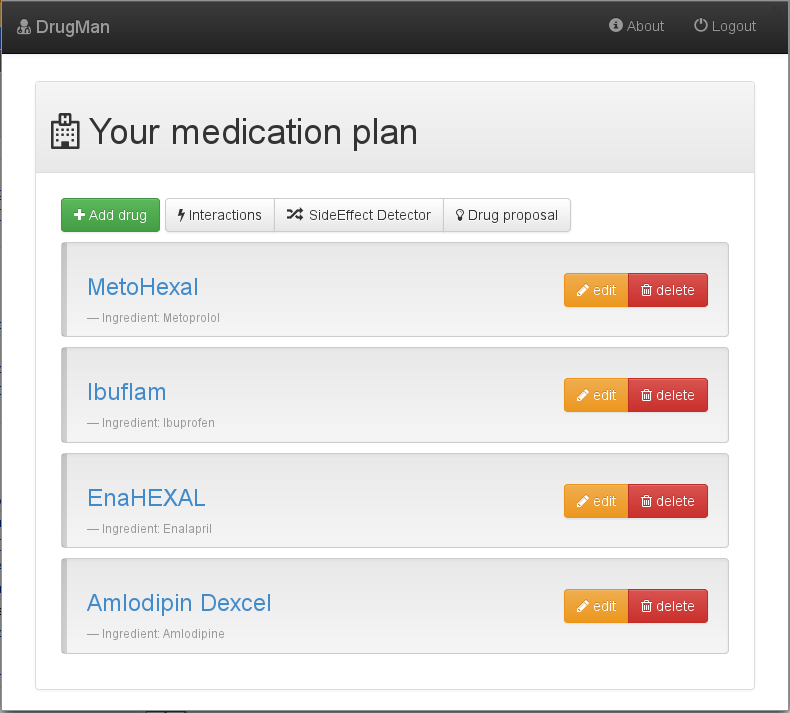
\includegraphics[scale=0.38]{evaluation/drugman}
  \caption{Screenshot of DrugMan}
  \label{fig:drugman}
\end{figure}

% \subsubsection*{User management}
% DrugMan implements a classic user management approach.
% The registration is open for everyone
\subsubsection*{Medication plan}
The central part of DrugMan is the medication plan.
Each registered user can add several drugs to their medication plan.
This allows the user always to have the overview of the current taken drugs.
A drug item of the medication plan consists of a label and an active ingredient.

\subsubsection*{Drug details}
The details page about a drug gathers different information about the drug and their active ingredient.
One example for such details are pharmacokinetic information about the active ingredient. 
Among others these information contains the absorption, route of elimination and the affected organism.
Other examples for details are side effects or available packagers and manufacturers.

\subsubsection*{Interactions}
The first of several actions that can be executed on top of the medication plan is a drug-drug interaction check.
This action will test all the drugs that are included in the medication plan for possible drug-drug interactions.
These checks are based on the active ingredient of each drug.
In case of existing interactions the affected drug-drug combination and some details about the interaction will be communicated by a notification.

\subsubsection*{Side effect detector}
Another feature is the ``Side effect detector''.
By specifying several side effects, the side effect detector will return all the drugs of the medication plan that may cause these side effects.
The process of specifying the side effects is supported by an autocomplete function that gathers side effects from the SIDER knowledge base.
The matching is done by comparing the given side effect URI's of the user with all the URI's of possible side effects of the drugs inside the medication plan.

\subsubsection*{Drug proposals}
The drug proposal feature supports the user by informing about possible drugs to a given disease.
After specifying a disease the user will get a selection of possible drugs.
Based on this selection the user can read some details about the drug including side effects, add this drug to the medication list or check whether the drug suits to the other drugs of the medication list in terms of possible drug-drug interactions.

\subsection{Integration of SEDRI}
\label{sec-2}
Since DrugMan was developed as a side project of this thesis the project is tightly coupled with SEDRI.
The internal architecture of DrugMan can be grouped in the management component and the drug specific component.

The former one is responsible for the general management features like user management including registering new users, login, logout etc. and the medication plan features including the registration, modification and deletion of drug items.

The latter component is responsible for the drug-specific features and is completely based on SEDRI.
This means all the funtionality described in Section \ref{sec:features} except the medication plan is built on top of SEDRI.

An example that SEDRI is usable for frontend information as well as backend processing is the Side effect detector.
This feature uses the side effects endpoint of SEDRI in the backend for the internal comparison of the given side effects and all the possible side effects of the current medication.
On the other hand it uses the same endpoint in the frontend by displaying all available side effects in the detail page of a drug.
If desired the application could request different return formats for the different use cases.
But in the case of the Side effect detector JSON-LD is used for both processes and the evaluation showed that this suits well.
%%% Local Variables: 
%%% mode: latex
%%% TeX-master: "../thesis"
%%% End: 



\chapter{Summary}
\label{cha:summary}




\chapter{Discussion}
\label{cha:discussion}



% Anhang
\appendix

% Quellcode
%\chapter{Quellcode des Systems}
%\rem{Quellcode-Link, zum Beispiel zum GitHub-Repo.}

% Literalturverzeichnis
\bibliographystyle{unsrt}
\bibliography{bibliography}
%\bibliographystyle{alpha}

\listoffigures
\listoftables
%\lstlistoflistings
%\listofalgorithms

% Erklärung
\clearpage
\pagestyle{empty}
\vspace*{1cm}
\begin{center}
\textbf{\sffamily Declaration}
\end{center}
\vspace*{0.5cm}
This master's thesis is the result of my own work. Material from the published or unpublished work of others, which is referred to in the thesis, is credited to the author in the text. I understand that failure to do this amounts to plagiarism and will be considered grounds for failure in this thesis and the degree examination as a whole.
% Ich versichere, dass ich die vorliegende Arbeit selbständig und nur unter Verwendung der angegebenen Quellen und Hilfsmittel angefertigt habe, insbesondere sind wörtliche oder sinngemäße Zitate als solche gekennzeichnet. Mir ist bekannt, dass Zu\-wider\-hand\-lung auch nachträglich zur Aberkennung des Abschlusses führen kann.

\vspace{2cm}
\noindent
Leipzig, 14. March 2013\hfill Signature

\end{document}
